\begin{outline-text-1}
\begin{xlarge}
\begin{center}
IBM Research 体験談
\end{center}
\end{xlarge}

\begin{note}
\begin{alignright}
Made by guicho2.71828 (Masataro Asai)
\end{alignright}
\end{note}
\end{outline-text-1}

\section{概要}
\label{sec-1}

岸本先生およびAdi と研究をしてきました

渡航先: アイルランド

渡航機関: 7/26-11/4

契約期間: 8/1-10/31

実際の契約期間: 8/2-10/28

実際の活動期間: 8/20-10/28

\section{アイルランド}
\label{sec-2}

\begin{container-fluid}
\begin{row-fluid}
\begin{span6}
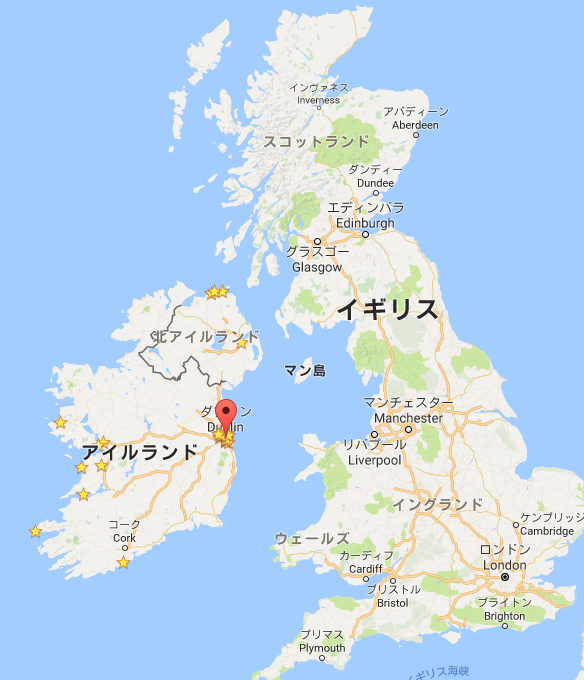
\includegraphics{img/static/ireland.png}
\end{span6}
\begin{span6}
\begin{itemize}
\item EU加盟国
\item 法人税回避のためIT企業が集結
\item 「ダブルアイリッシュ・ダッチサンドイッチ」
\item 気候: 冷涼,にわか雨↔曇りの繰り返し,太陽低い,≈イギリス
\item 人の性格: 大雑把
\end{itemize}
\end{span6}
\end{row-fluid}
\end{container-fluid}

\section{申し込みの流れ}
\label{sec-3}

\begin{itemize}
\item ? : メンター(例:岸本先生)がインターンシップの計画を作り会社に提出
\item 2015/6  : 知り合った人にポスト無いかどうか尋ねておく (事前に根回し)
\item 2015/12 : 応募の掲示
\item 2016/3:  応募の最終期限 ただし埋まり次第決定
\item 2015/12:  その企業の Job Opportunity ウェブサイトから登録
\item 何段階かの審査を経る(二ヶ月ぐらいかかる)
\item 審査を通ると、自分の名前、経歴等が社内のどこかに掲示されるらしい
\item メンターが気に入った人を選ぶ --- 根回しがここで効く。ただし採用されるかは不明
\item 2016/2: 最終面接 (国際電話)
\end{itemize}

\section{採用後の流れ}
\label{sec-4}

\begin{itemize}
\item Visa関連 -- 日本人はアイルランド入国に関しVISAはいらない
\item Hosting Agreement -- 就労許可を得るためのEU/アイルランドのシステムの1つ。
\begin{itemize}
\item 国際郵便がロストしたので直前に送り直しなど
\end{itemize}
\item 契約書
\begin{itemize}
\item 郵送+メール
\end{itemize}
\item 国内手続き
\end{itemize}

\section{国内手続き}
\label{sec-5}

\begin{itemize}
\item 国内(JSPS) = ヤクザの親分
\begin{itemize}
\item 多数の手続きを設けることで国際化を妨害
\item 3ヶ月以上の海外渡航を認めない
\item →本来4ヶ月のインターンを短縮することに
\end{itemize}
\item 国内(大学)
\begin{itemize}
\item 契約書を二週間で返信しないといけない
\item 来月の教授会まで待て? 今日やれ今日
\item confidentialな契約書の内容を見せろ?
\end{itemize}
\item 国内(学科) (略)

\item 結論: センスの悪い人間/技術/組織と関わりを持つのは時間の無駄

\item 結論: Lisp で書け
\end{itemize}

\section{準備(持ち物): アウトドア/ノマド生活を基本に。}
\label{sec-6}

\begin{itemize}
\item 夏服、冬服
\item 調理器具 ← アウトドア用の食器がおすすめ。コンパクトにフライパン、鍋、皿を収納
\item 調味料 ← めんつゆ, わさび
\item プログラミング環境。
\begin{itemize}
\item Hackers = Painters. 能力を最高に保つため 慣れ親しんだ道具を確保するのはプロの責務。
\item \textbf{キーボード} ← プログラマにとって指と手は命。
\item \textbf{ディスプレイ} ← 必ずセカンドディスプレイをもらえるとは考えない
\item \textbf{工具} ← 最低限自分のノートパソコンを修理できるだけの工具
\end{itemize}
\end{itemize}

\subsection{写真}
\label{sec-6-1}

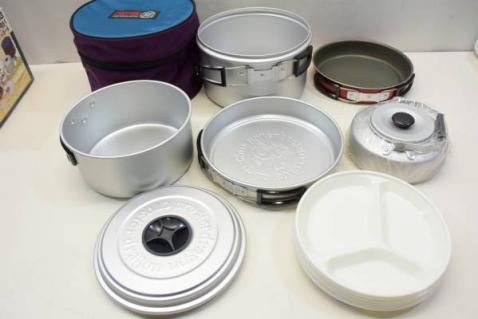
\includegraphics{img/static/cooker.jpg}

\subsection{写真}
\label{sec-6-2}

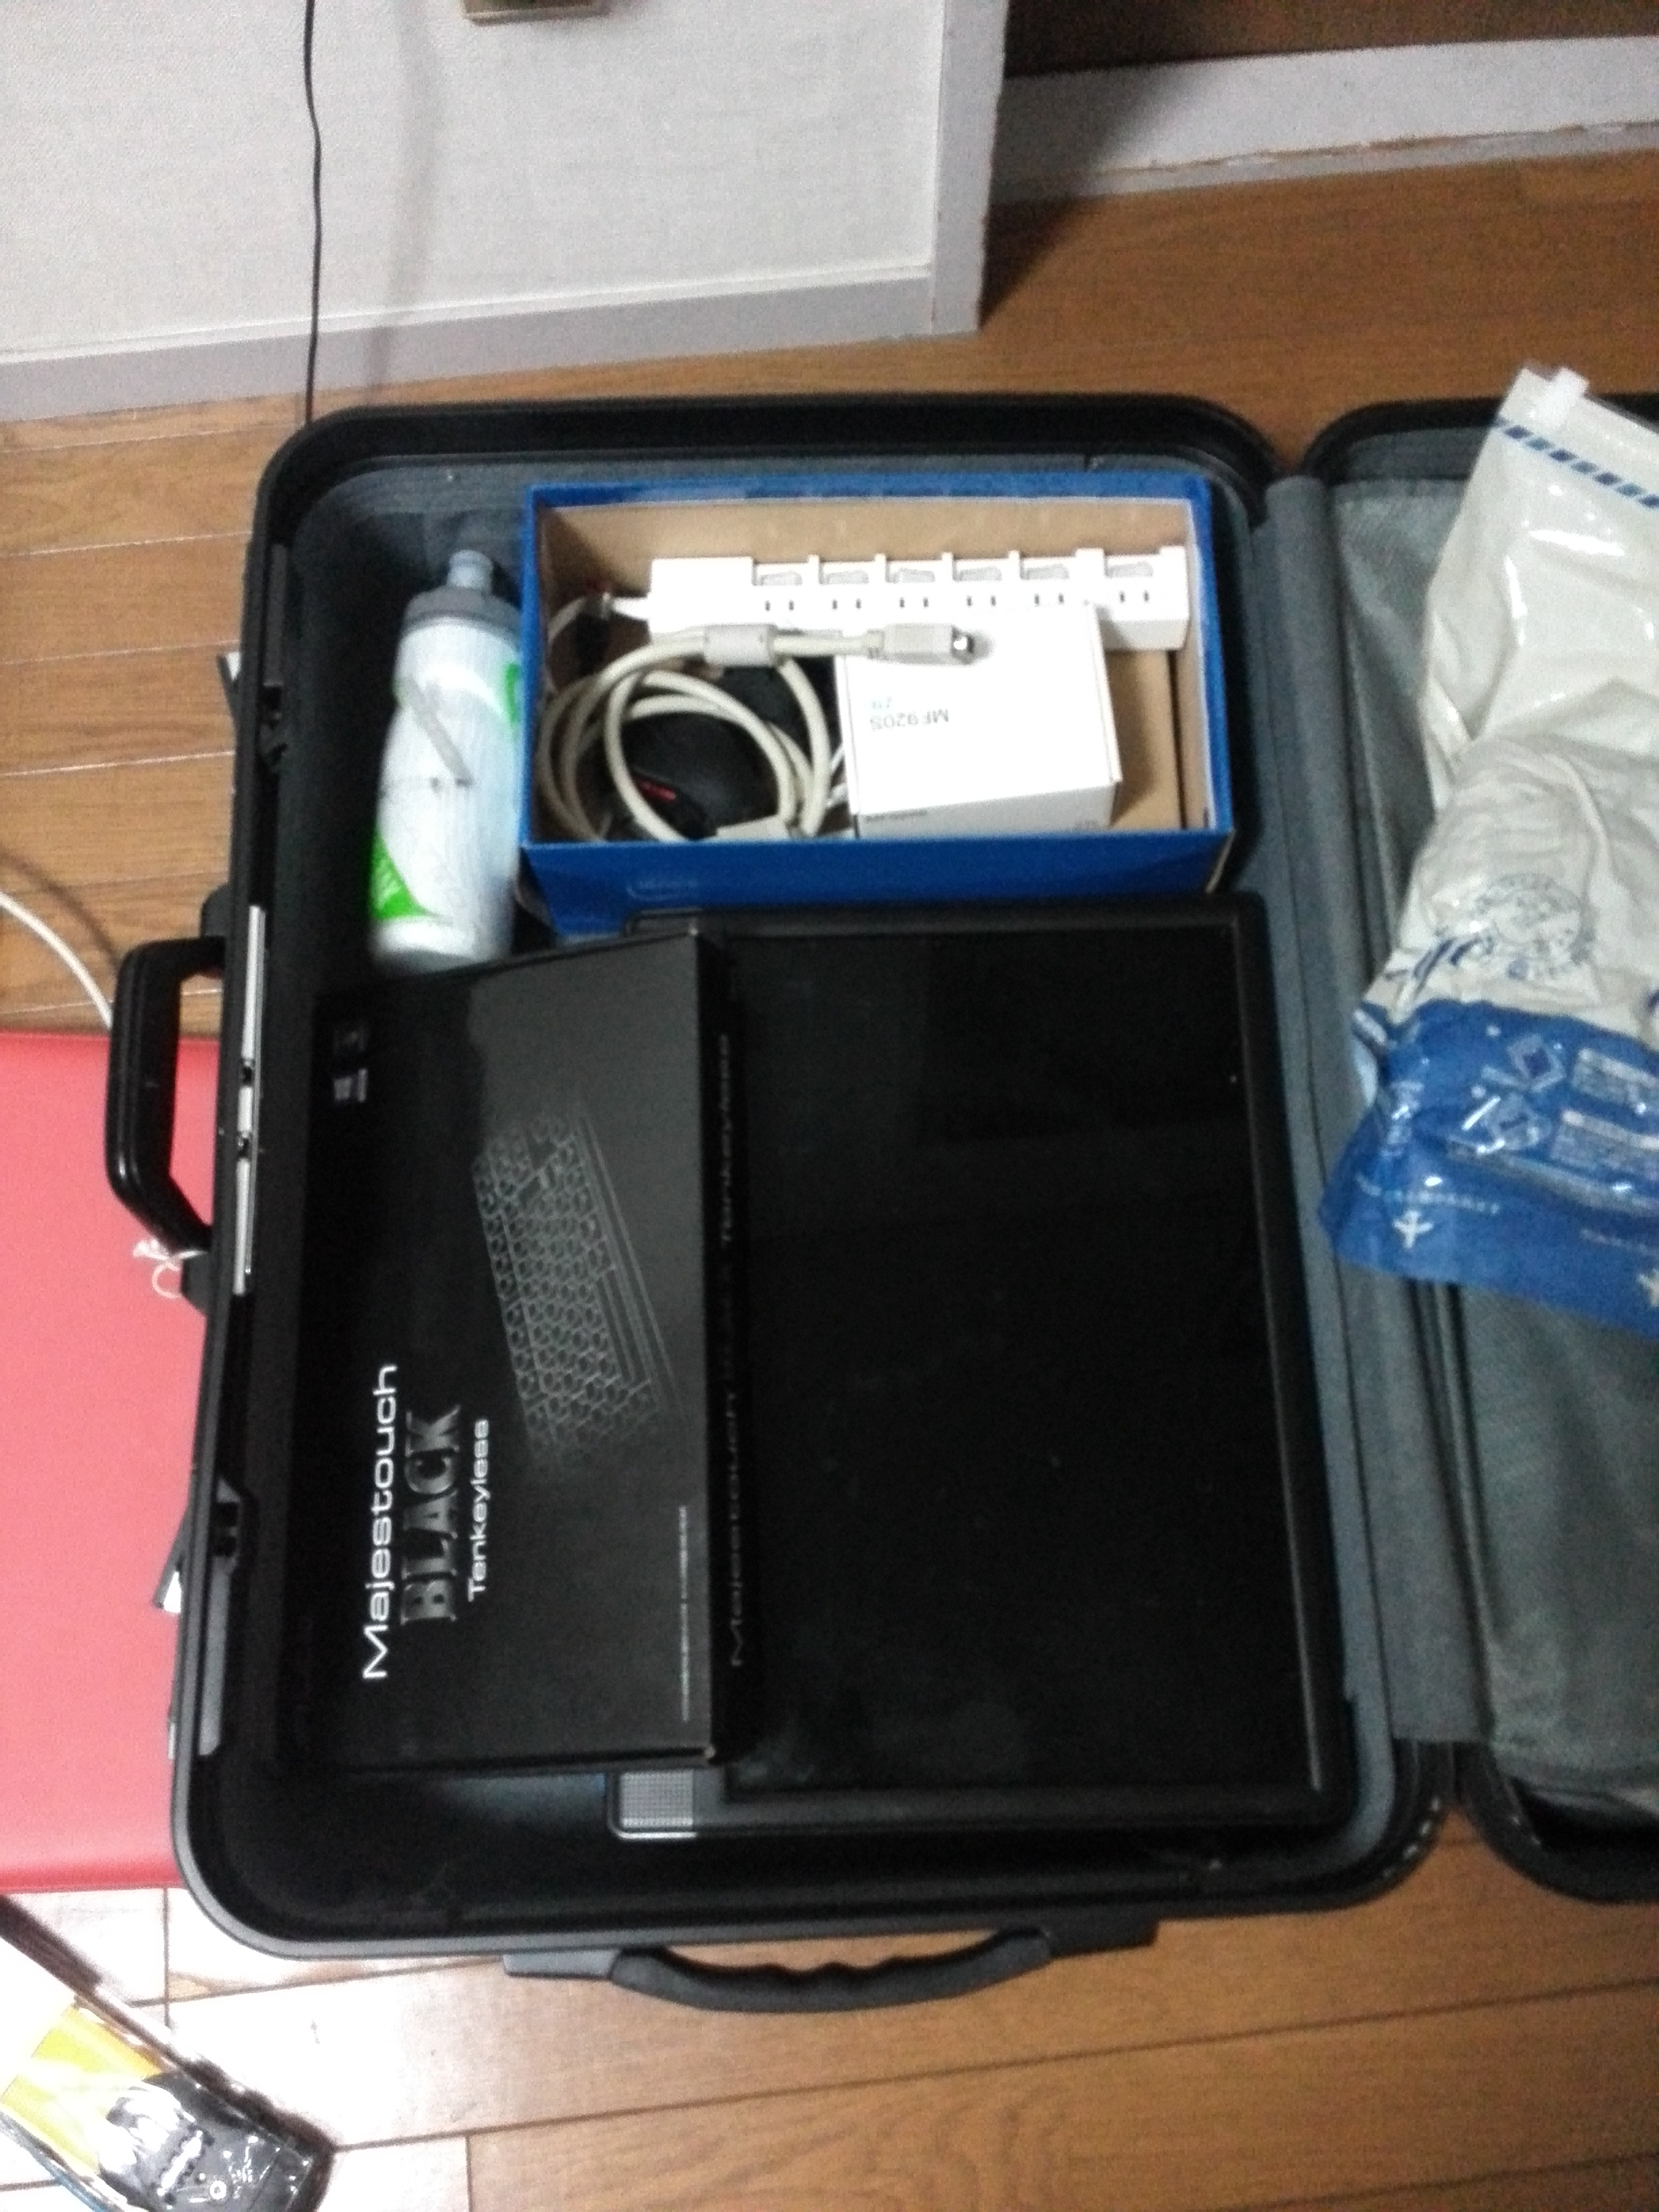
\includegraphics{img/static/display.jpg}

\subsection{写真}
\label{sec-6-3}

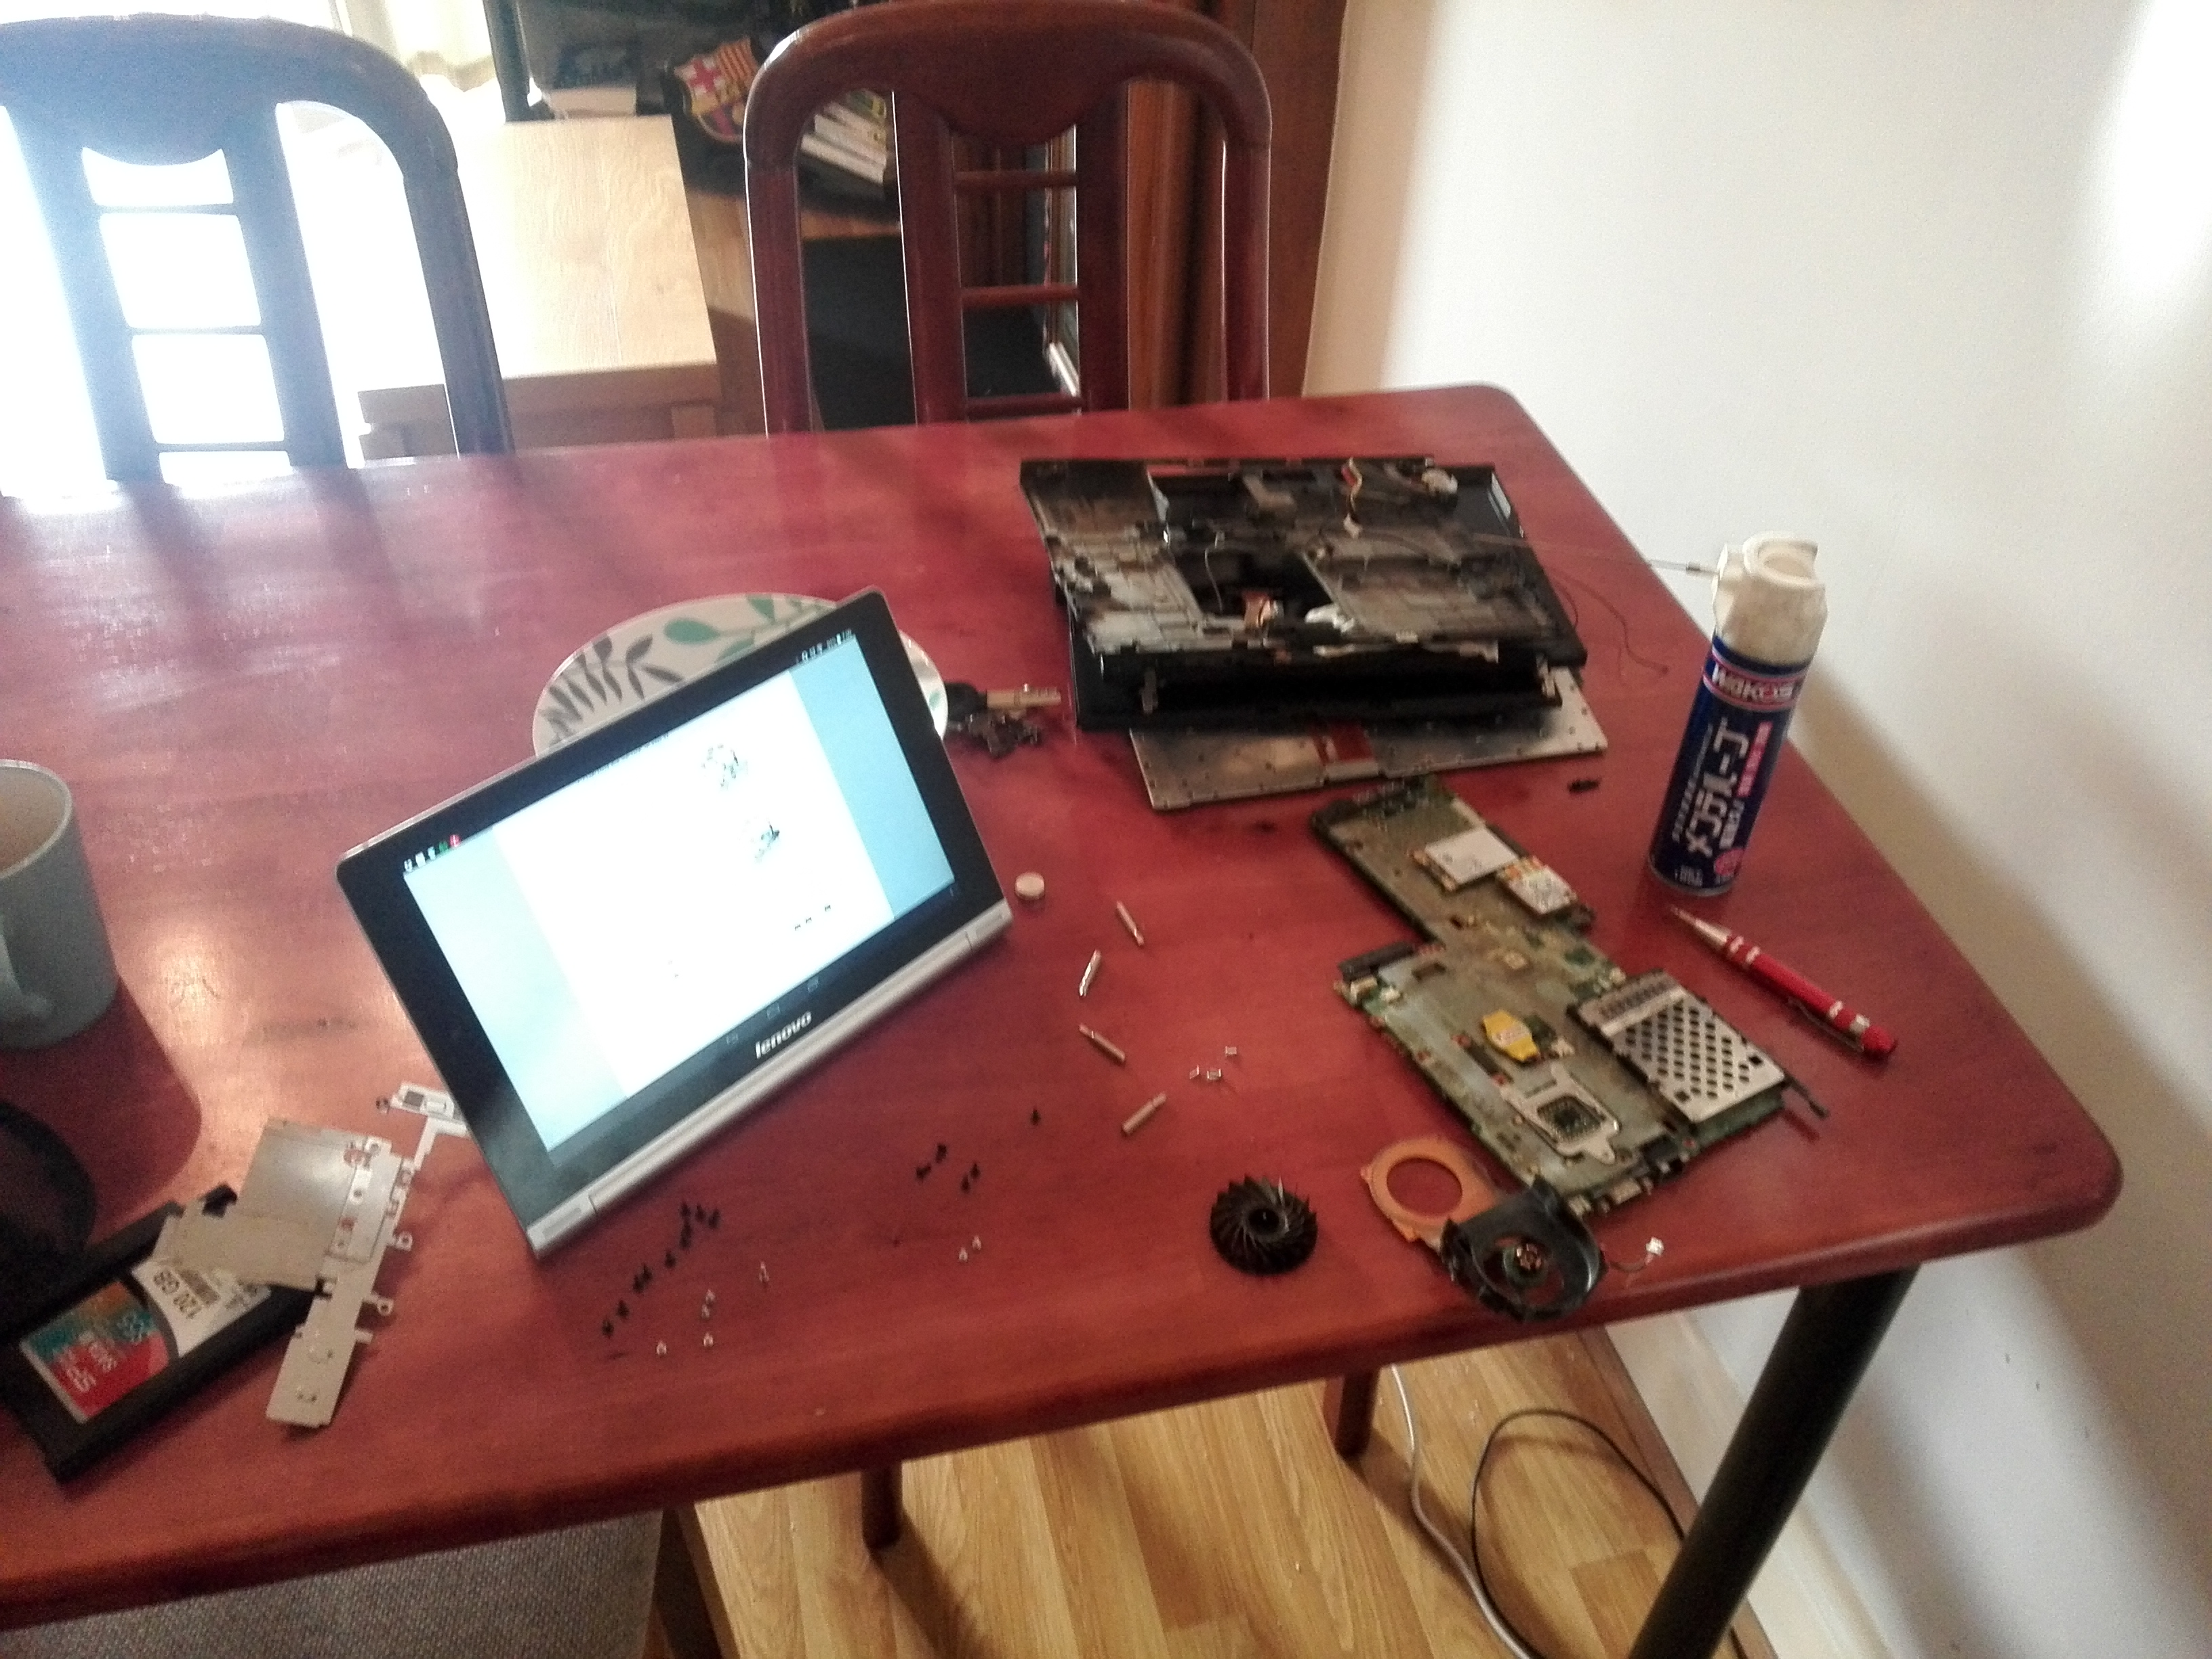
\includegraphics{img/static/fix.jpg}

\section{準備(住居): Airbnb 最高!!!}
\label{sec-7}

\begin{center}
\begin{tabular}{lll}
期間 & 場所 & Approx. JPY/day\\
\hline
7/26-8/04 & 南ダブリン, Airbnb, 部屋の片隅のベッド & 4k\\
-9/4 & ダブリン市内, Daft.ie, 三人部屋二段ベッド上 & 1.3k (500EUR/month)\\
-10/31 & ダブリン郊外, Airbnb, 個室 & 2.4k (800EUR/month)\\
11/1 & Galway, Airbnb, 個室 & 3.6k\\
11/2 & Belfast UK, Airbnb, 個室 & 3.8k\\
11/3 & Dublin, Airbnb, 個室 & 3.9k\\
\end{tabular}
\end{center}

\subsection{同居人}
\label{sec-7-1}

\begin{center}
\begin{tabular}{llll}
期間 & 場所 &  & \\
\hline
7/26-8/04 & 部屋の片隅のベッド & Venezuera & \\
 &  & German & \\
 &  & Taiwan & \\
\hline
-9/4 & 三人部屋二段ベッド上 & Spain & China\\
 & 9-10人で集団生活 & Italy & Brazil\\
 &  & France & Russia\\
 &  & Libya & \\
\hline
-10/31 & 個室 & Italy & Croatia\\
 & 3-4人で集団生活 & France & Estonia\\
\end{tabular}
\end{center}

\subsection{部屋 (ダブリン市内)}
\label{sec-7-2}

\includegraphics{img/static/patric.jpg}

\subsection{部屋 (ダブリン郊外)}
\label{sec-7-3}

\includegraphics{img/static/ingram.jpg}

\subsection{部屋 (ダブリン郊外) Charlie}
\label{sec-7-4}

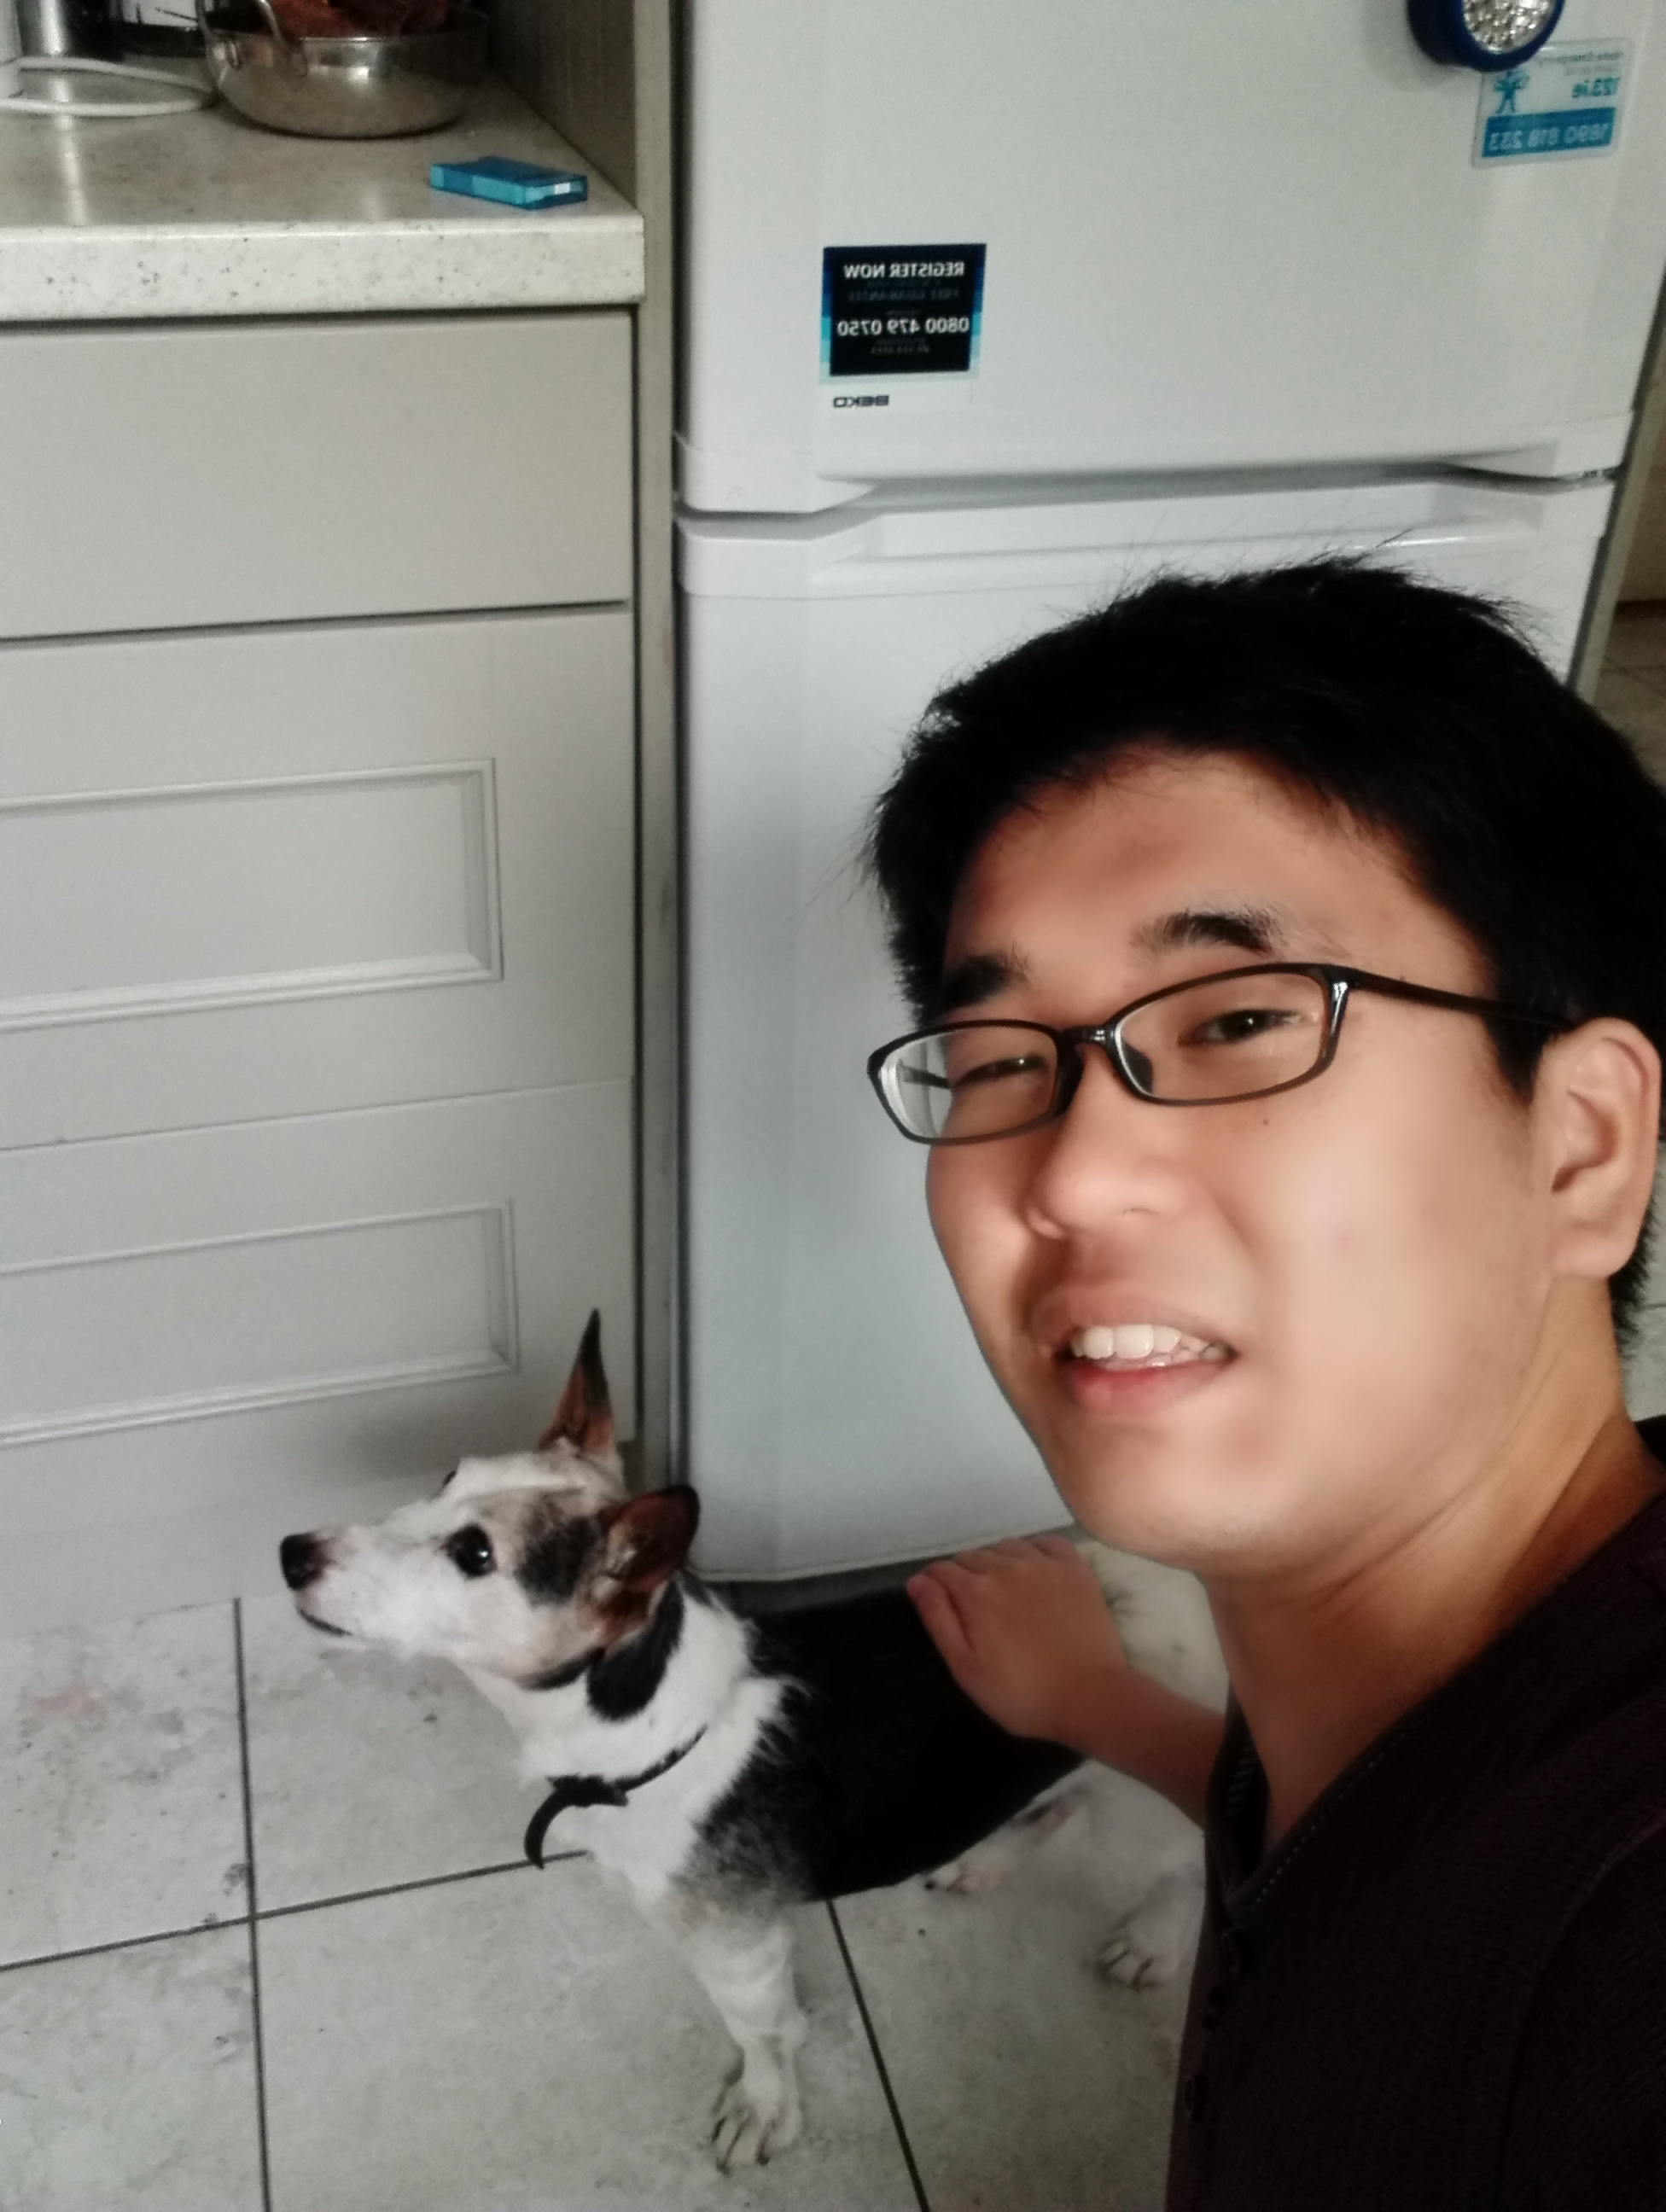
\includegraphics{img/static/charlie.jpg}

\subsection{ルームメイト (ダブリン市内)}
\label{sec-7-5}

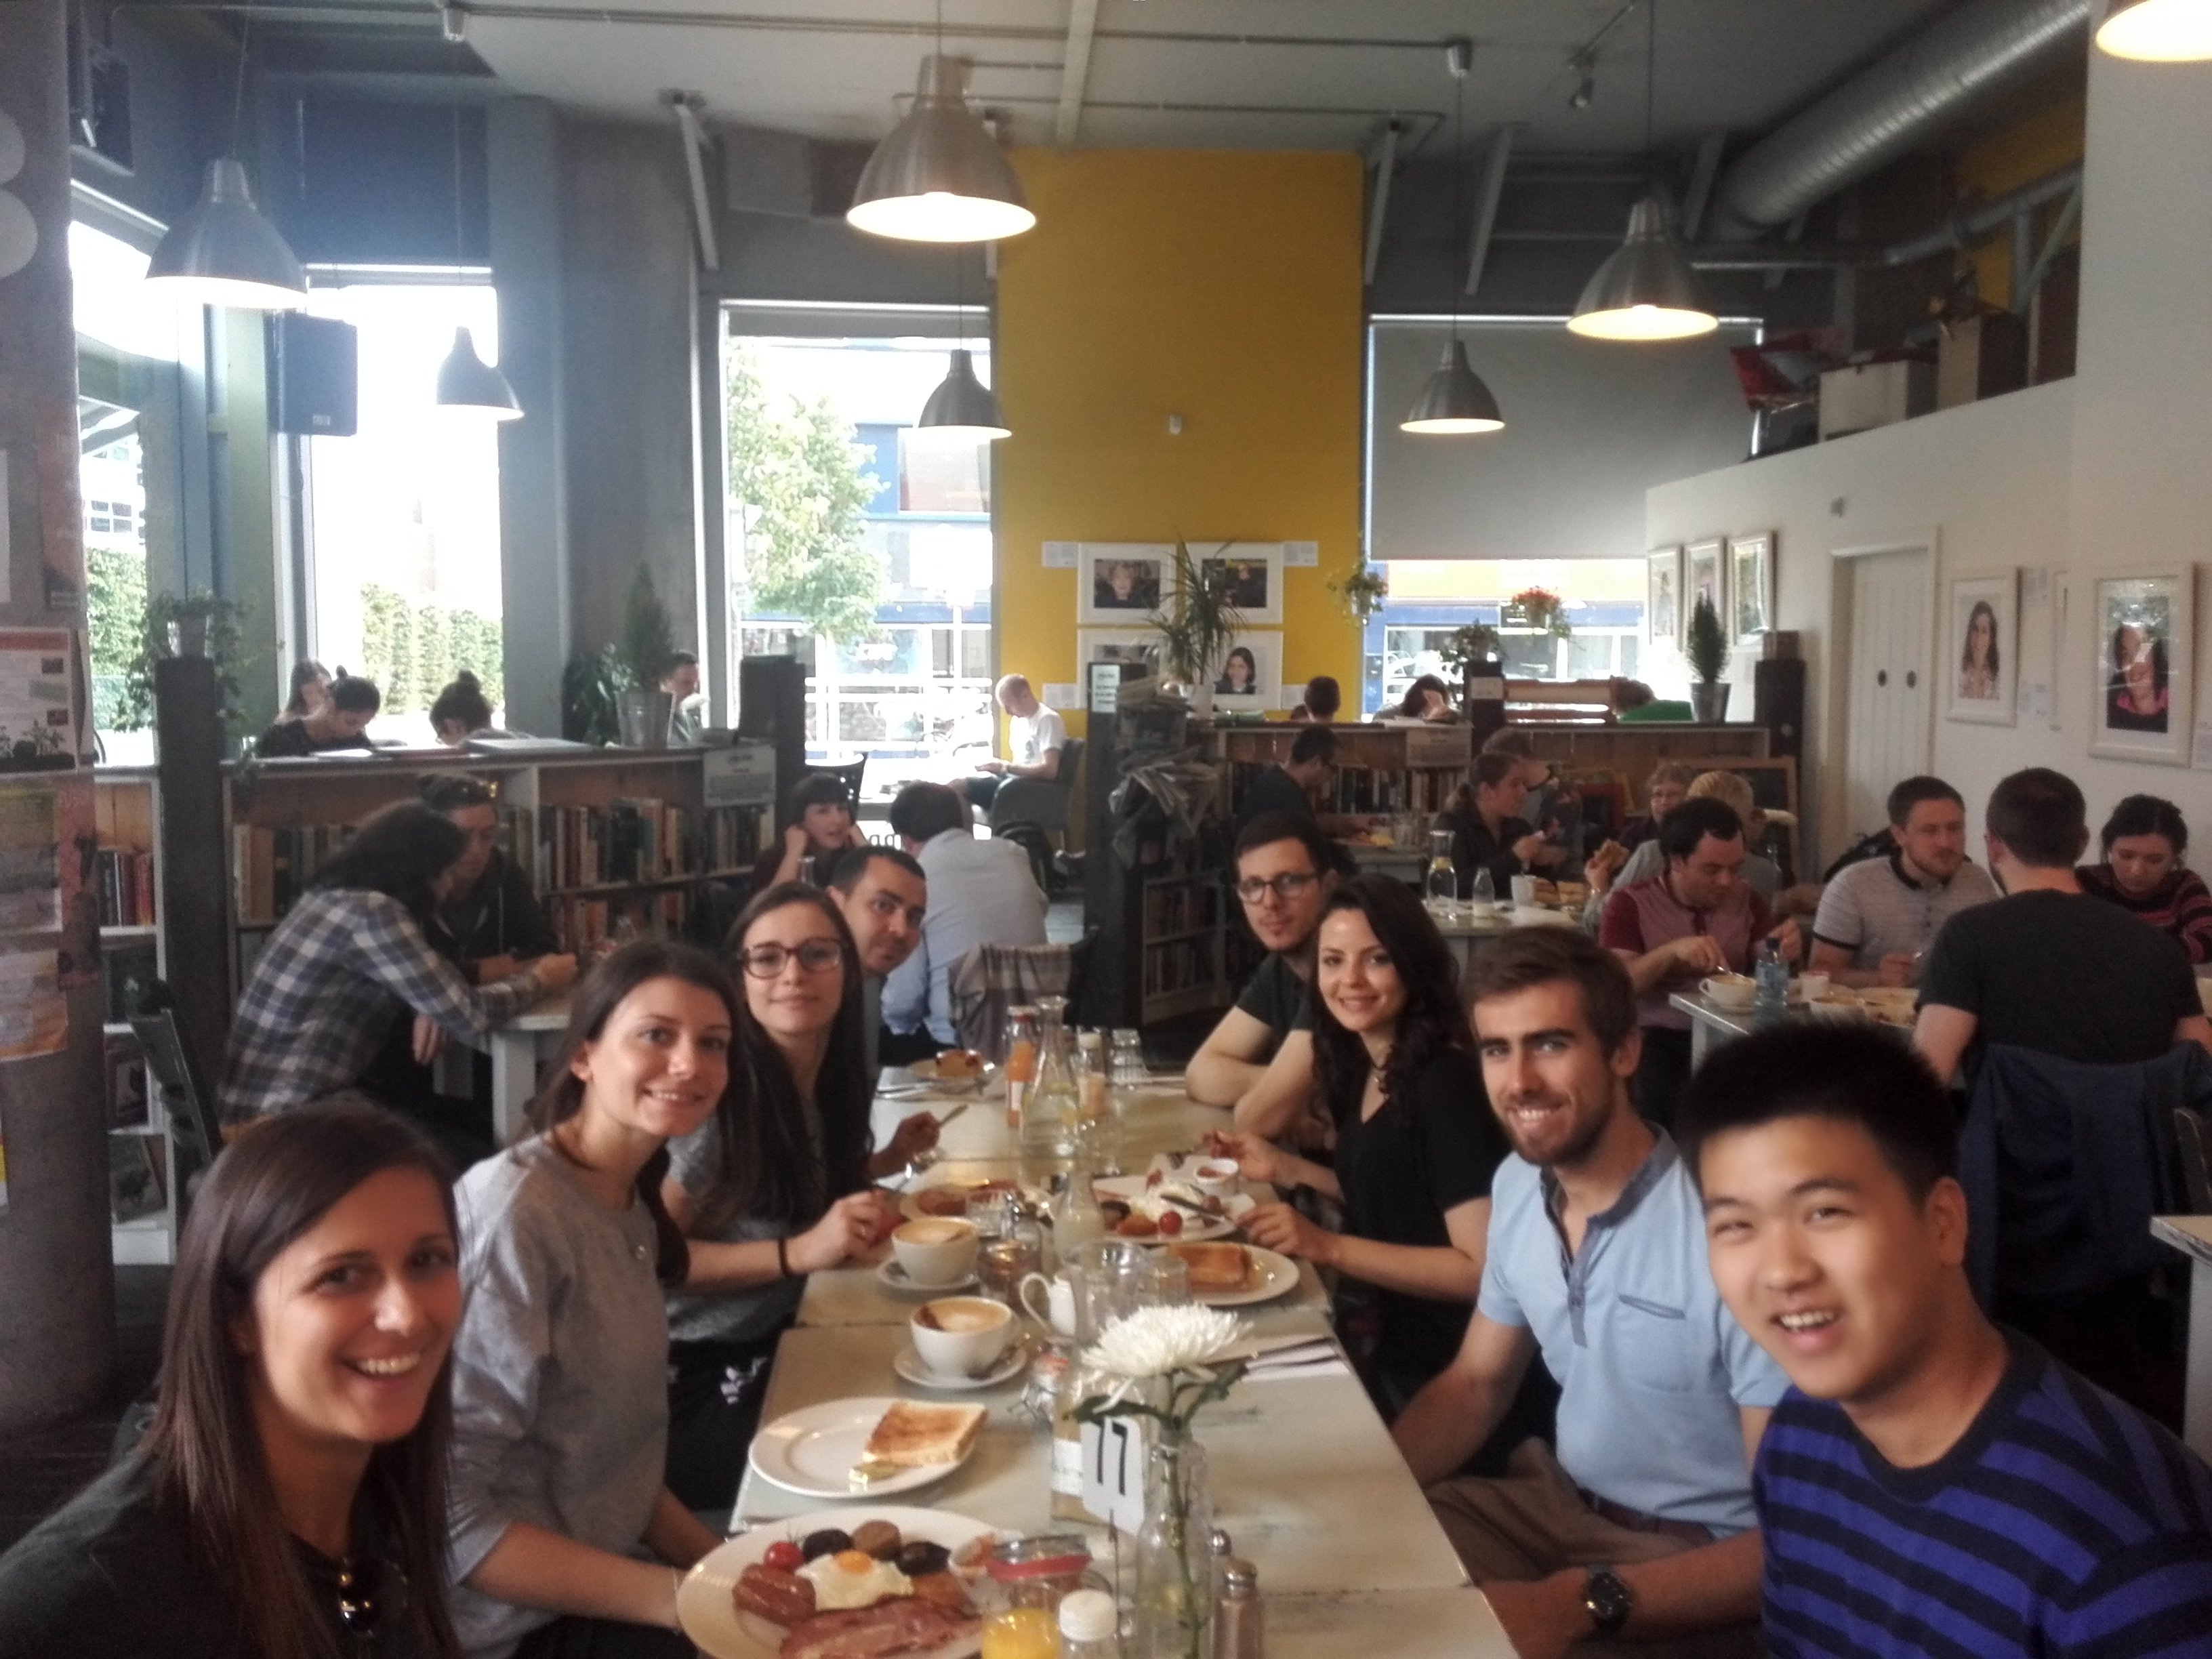
\includegraphics{img/static/roommates.jpg}

\subsection{ルームメイト (ダブリン郊外)}
\label{sec-7-6}

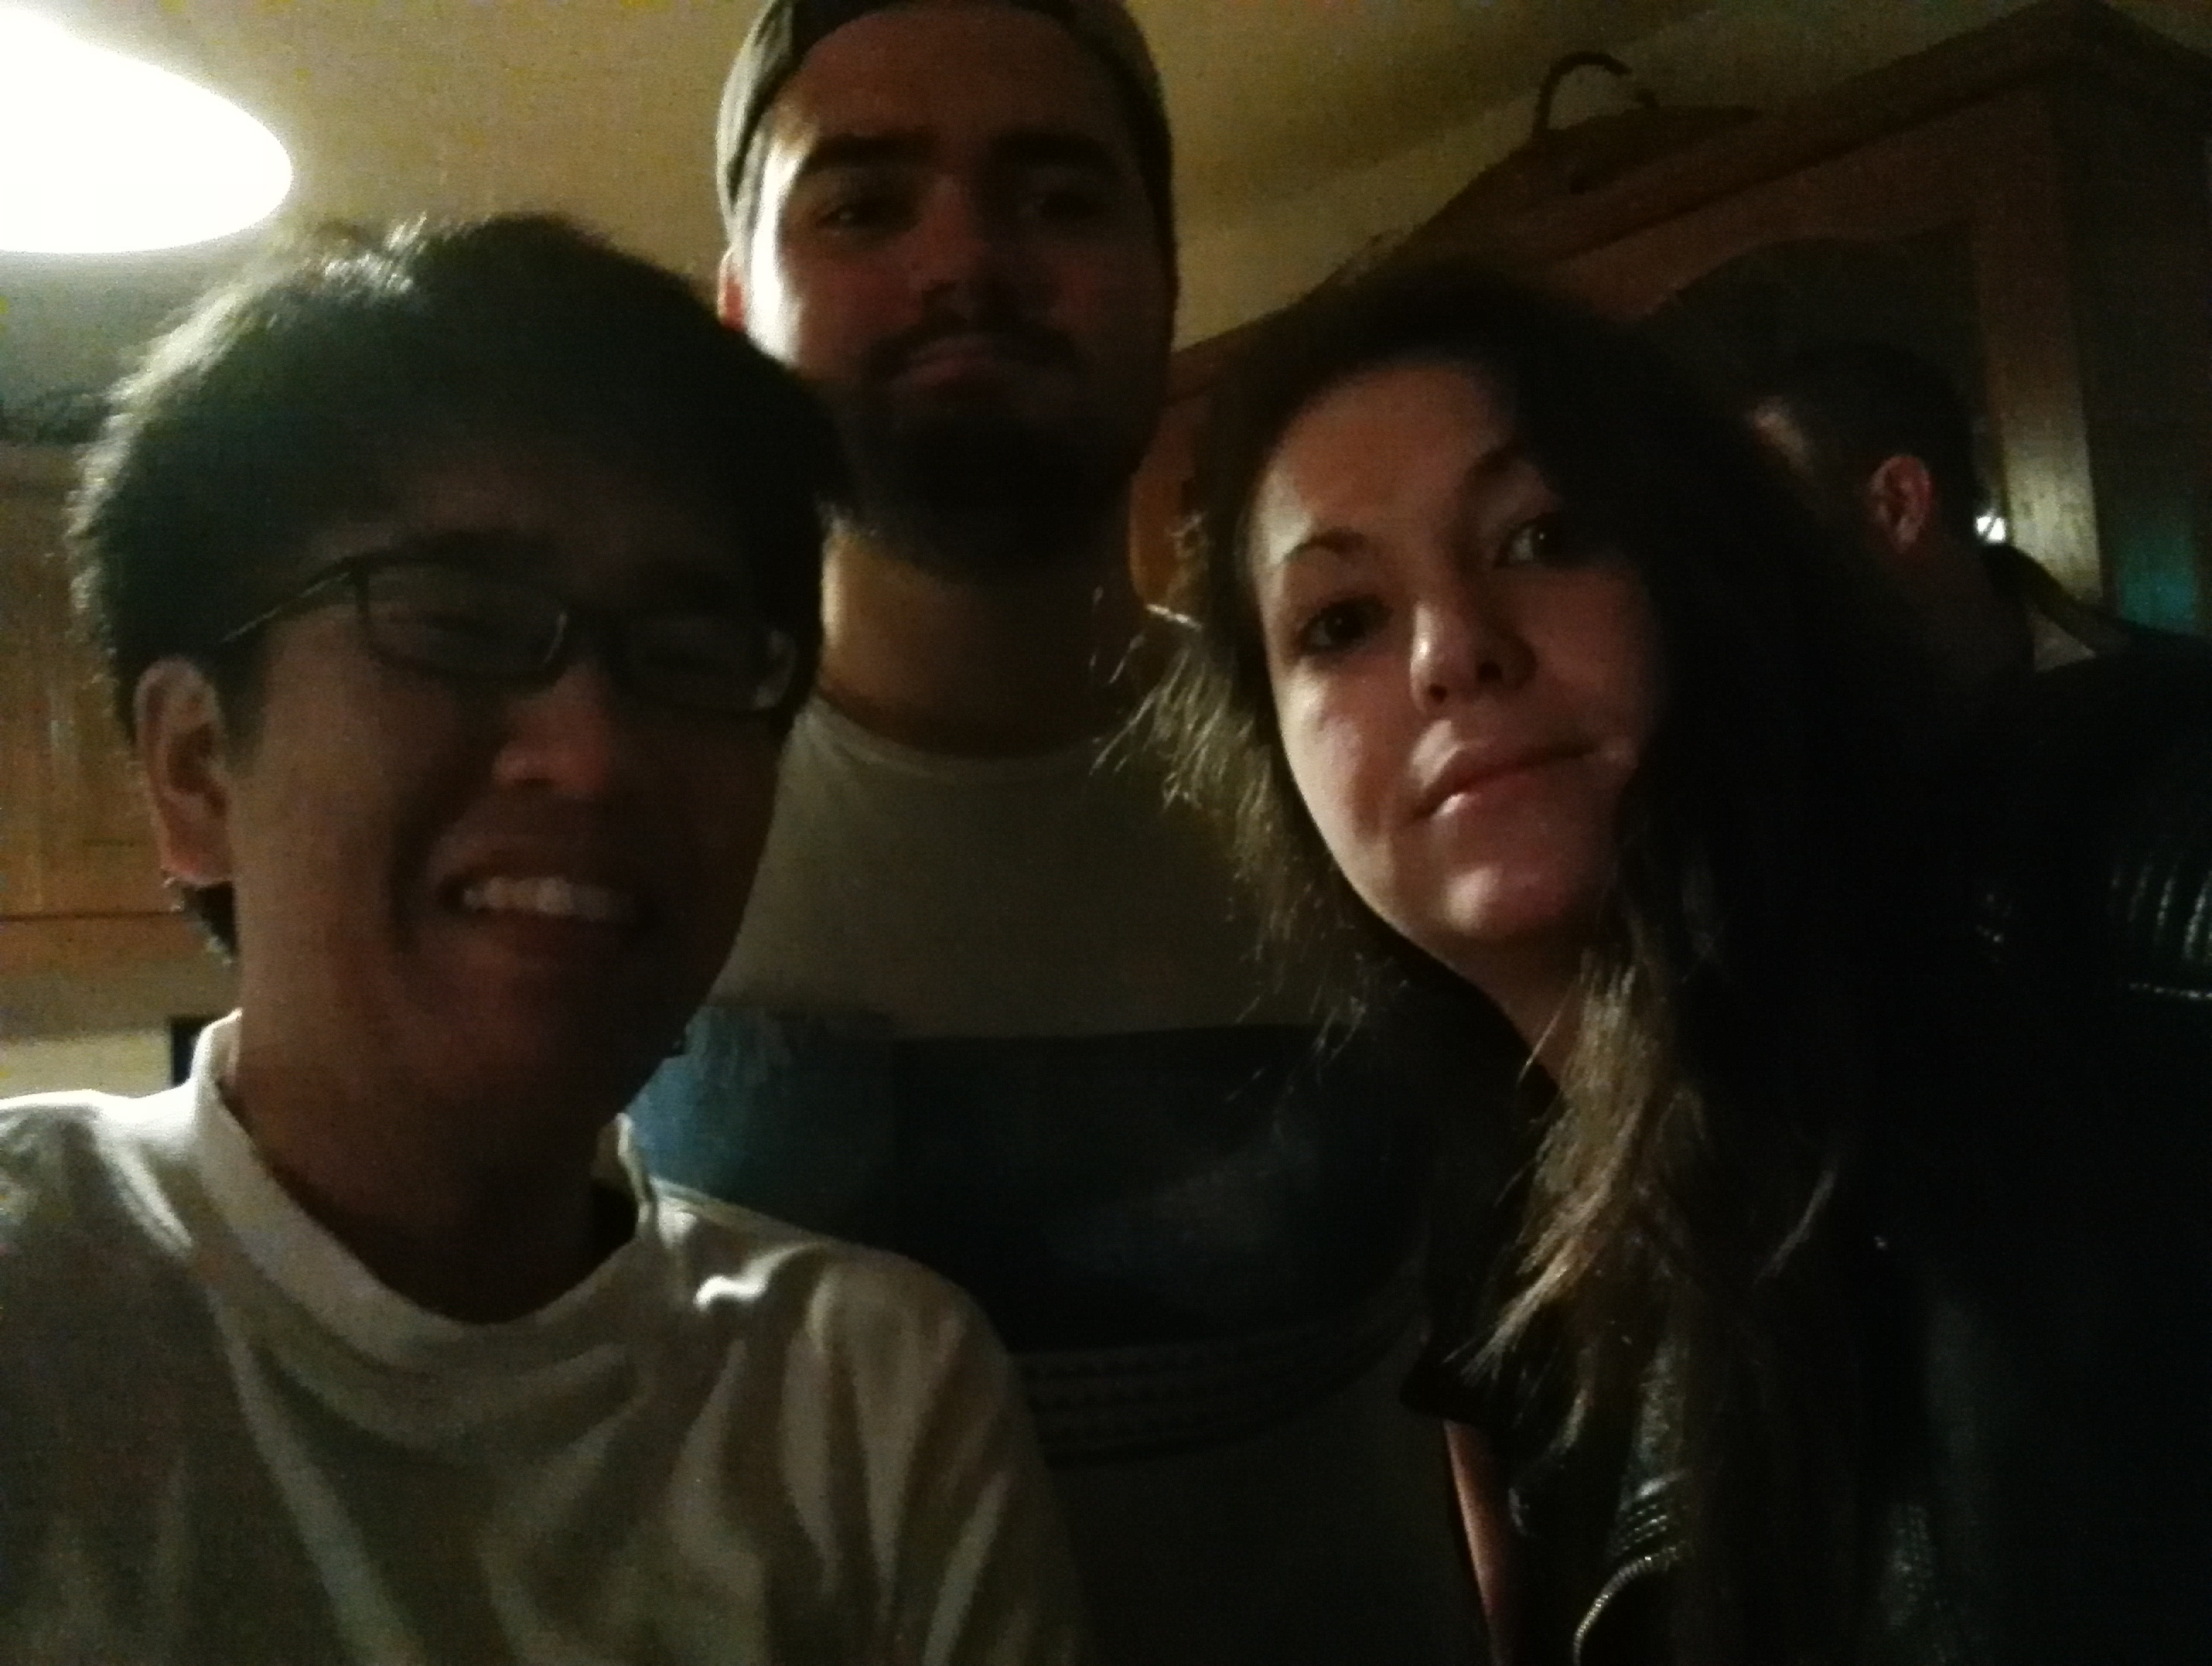
\includegraphics{img/static/iralia.jpg}

\subsection{ルームメイト (ダブリン郊外)}
\label{sec-7-7}

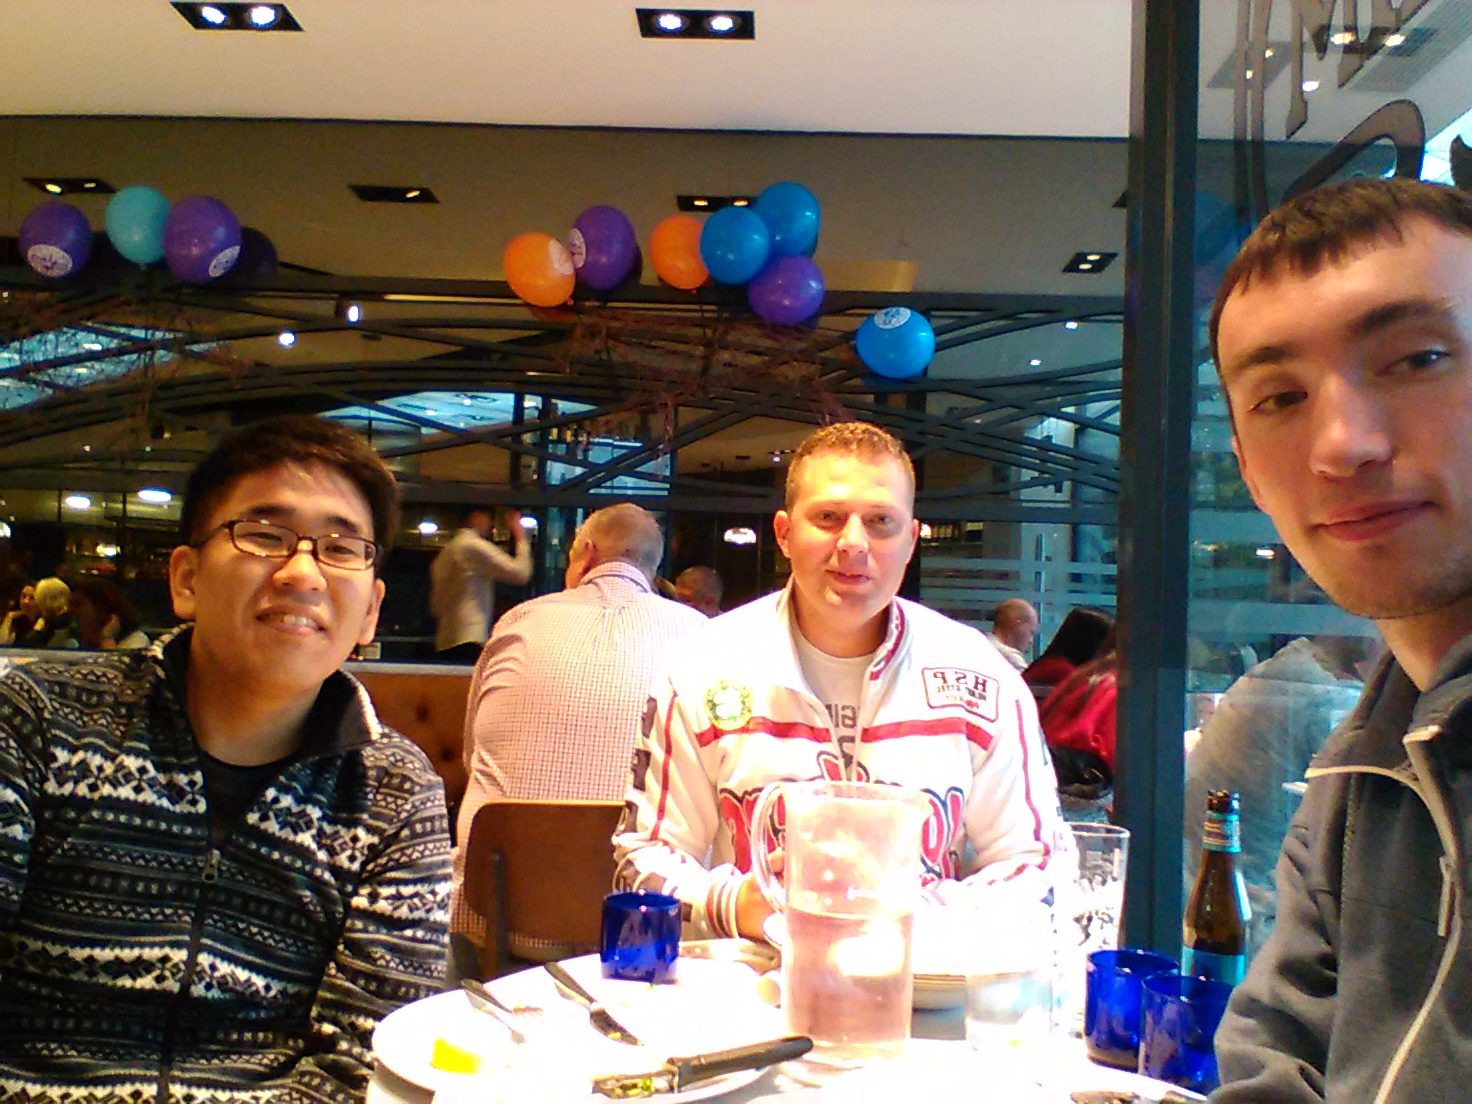
\includegraphics{img/static/andrei.jpg}

\section{IBM Research Ireland}
\label{sec-8}


\includegraphics{img/static/campus.png}

\section{IBM Research Ireland}
\label{sec-9}


\includegraphics{img/campus-fake.png}

\section{環境}
\label{sec-10}

食堂は不味い/2時に閉まる/売店なし/周囲に何もない

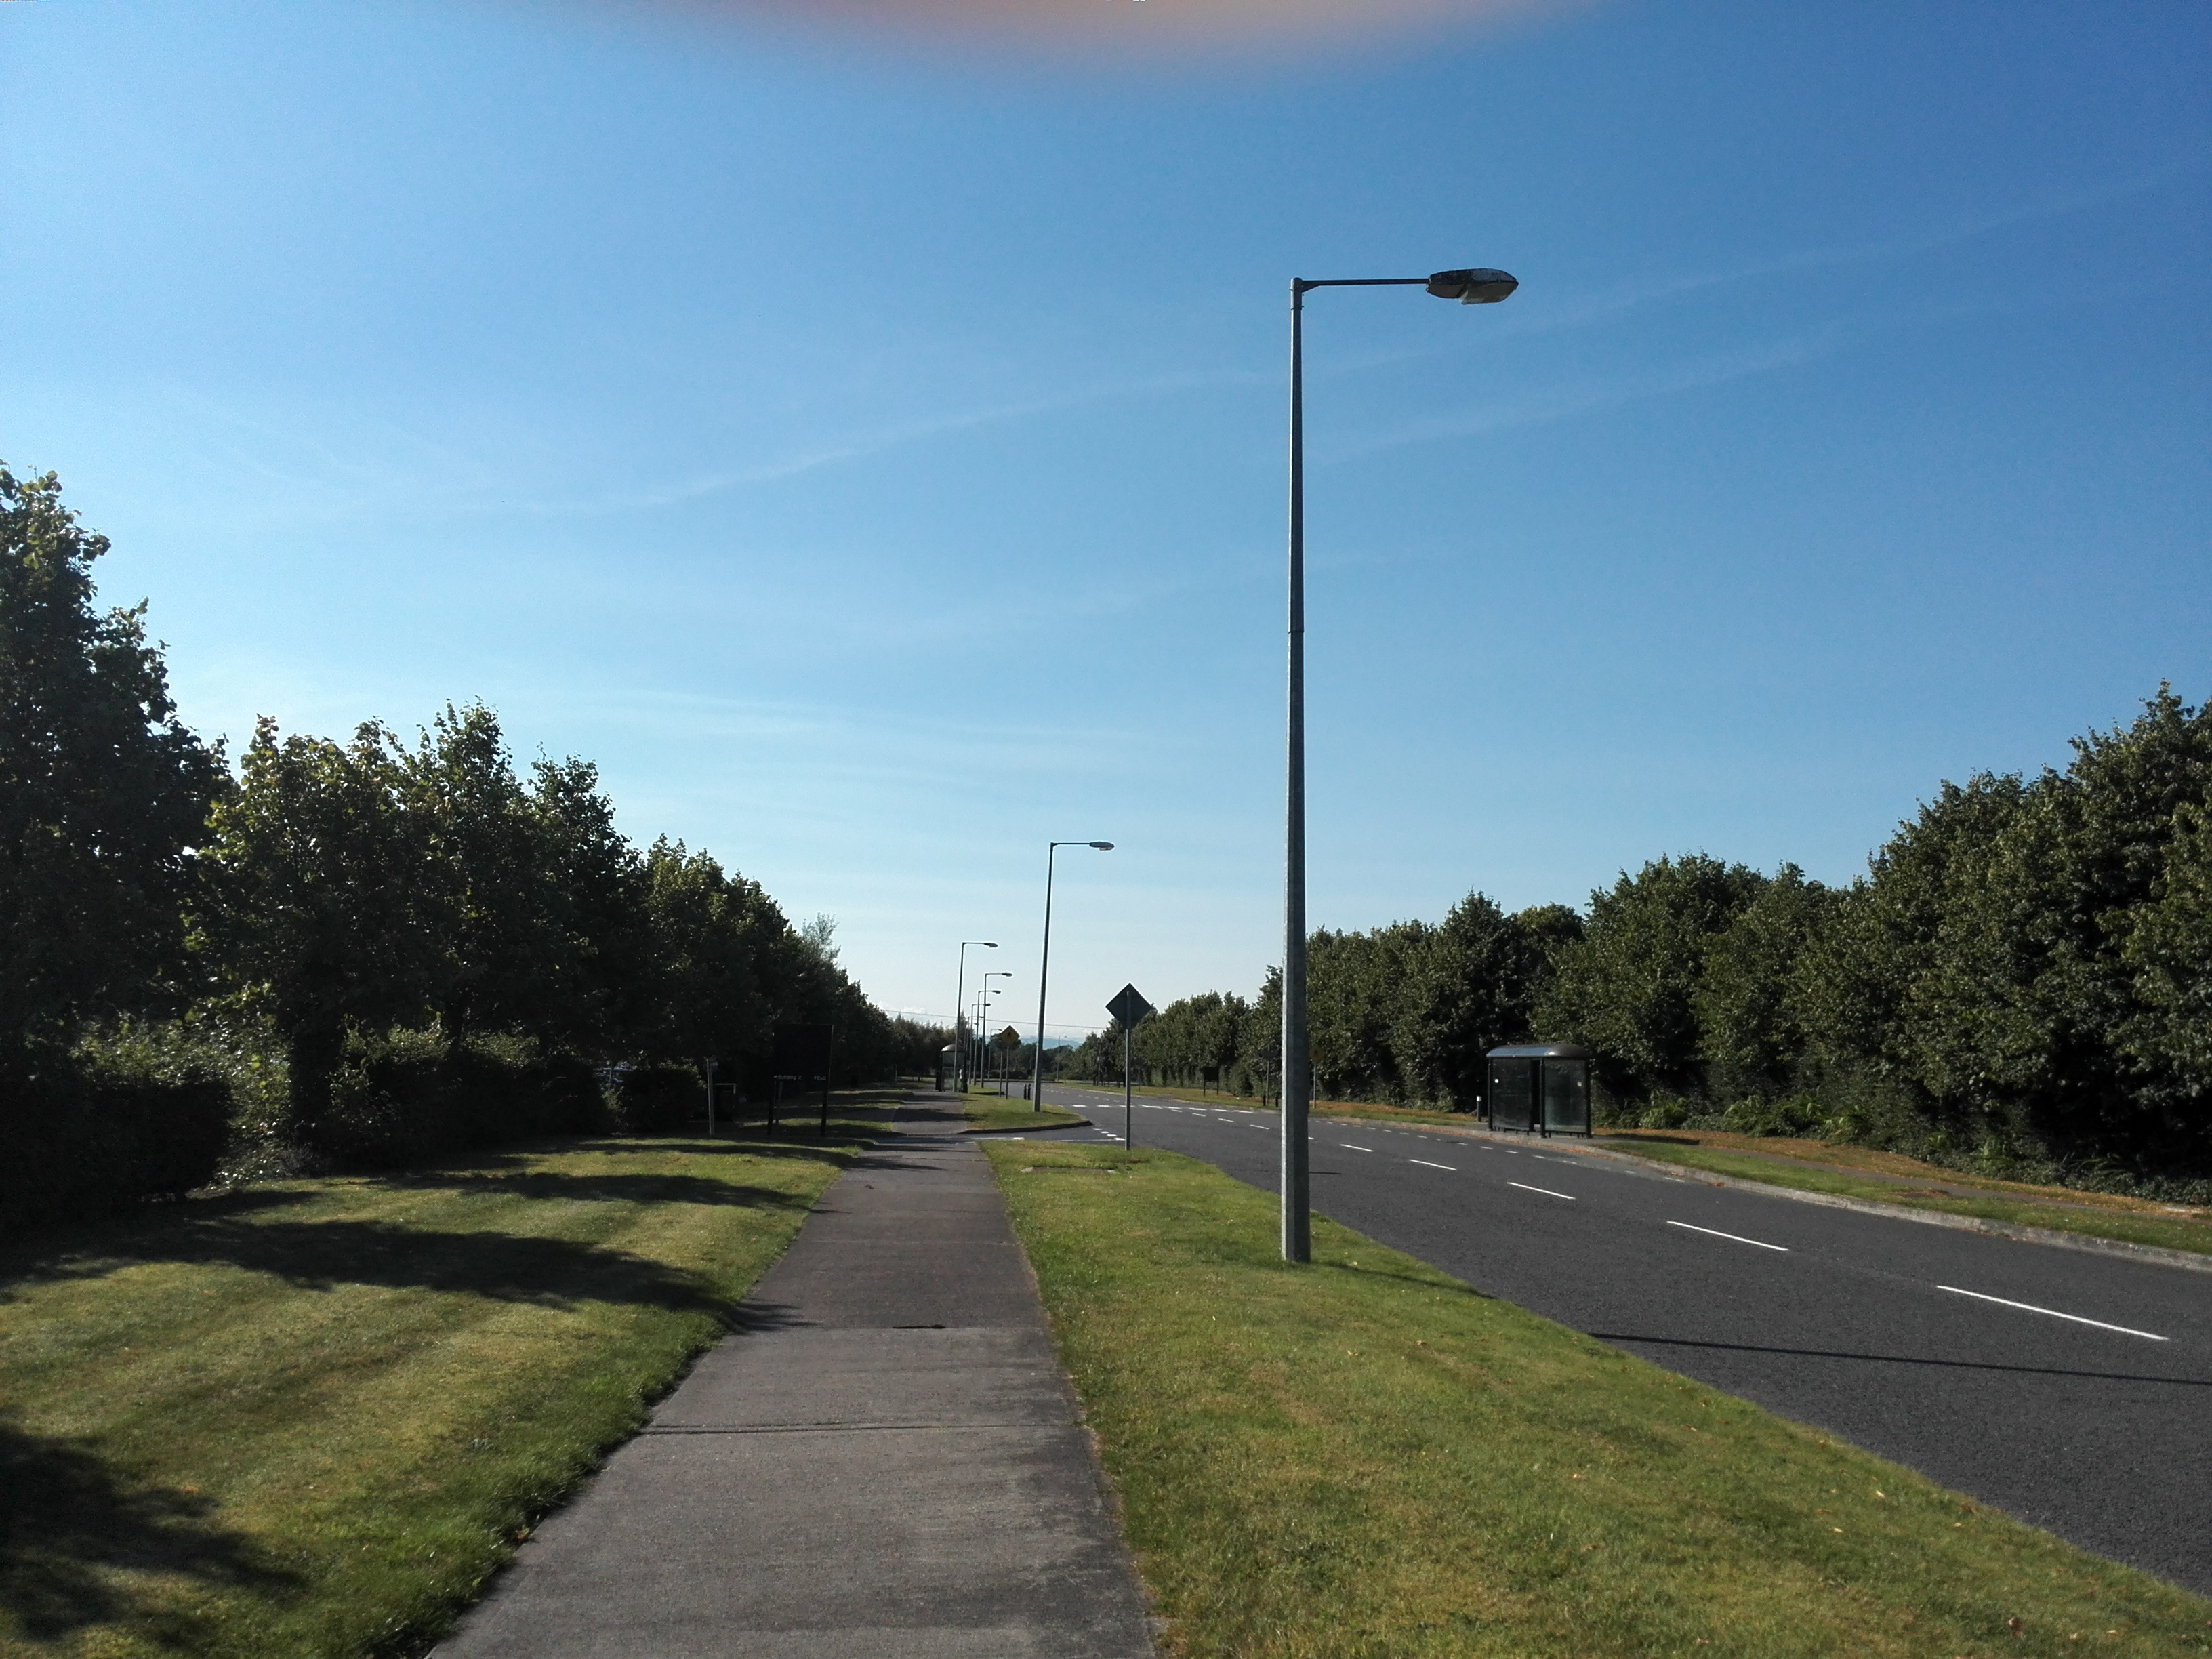
\includegraphics{img/static/nothing.jpg}

\section{到着後}
\label{sec-11}

\begin{center}
\begin{tabular}{ll}
日時 & \\
\hline
7/26 & 到着\\
7/29 & 移民登録 (350€ -- 自費)\\
8/2 & 始めてキャンパス内に\\
\textasciitilde{}8/9 & ようやくイントラネットアカウント\\
 & =インターネットアクセス\\
 & =apt-get で開発環境を構築\\
\textasciitilde{}8/20 & ようやくサーバーアカウント\\
 & まともに開発できるようになる\\
\end{tabular}
\end{center}

実質まともに開発できたのは二ヶ月ちょい

\section{病的な既存コード}
\label{sec-12}

\begin{itemize}
\item テスト無し CI無し ドキュメント無し
\item コードレビュー無し スタイル統一無し
\item ビルドできない古い無数のサブプロジェクト, それらのためだけの関数
\item 不適切なクラス構造, switch 文, 不適切なメソッド名, もはや呼ばれていない関数
\item 手でJSON書き出し (しかも間違ってる)
\item インスタンスをコピーするのにそのJSONに書き出して読み込む
\end{itemize}

まともなプロセス間APIを手に入れるためのリファクタリングに一ヶ月 (研究できず)

実質まともに研究できたのは一ヶ月 (他のチームはまともなコードなのに…)

\section{救い}
\label{sec-13}

\begin{itemize}
\item \textbf{他のチームは} もっと現代的な環境で開発してる
\item 社内に github enterprise がある
\item Travis-CI enterprise もある
\item → 自分でCIをセットアップした
\item → 自動テストも書いた
\item → 古いコードは全部捨て
\item → 残りをリファクタリング
\end{itemize}

\section{給料}
\label{sec-14}

\begin{container-fluid}
\begin{row-fluid}
\begin{span6}
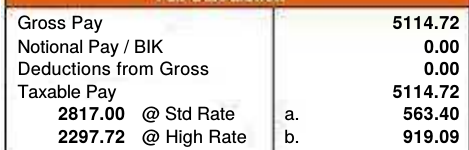
\includegraphics{img/static/pay.png}

\begin{itemize}
\item 最初の1ヶ月:45\% (Emergency Tax)

\item 残り2ヶ月: 20\%

\item 月22万 - 住居8万 = 14万

\item 交通費、食事\ldots{}

\item 航空券16万, 移民登録 3万5千
\end{itemize}
\end{span6}
\begin{span6}
\textbf{アイルランド固有の事情}

\begin{itemize}
\item 統一賃金支払いシステム: PAYE Anytime
\item PAYE Anytime の支払いはアイルランドの銀行のみ \textbf{WTF}
\item 現地銀行口座を開設するまで給料を貰えない
\item 現金を用意しておかないと一文無しに!
\end{itemize}
\end{span6}
\end{row-fluid}
\end{container-fluid}

\section{働きかた}
\label{sec-15}


\begin{container-fluid}
\begin{row-fluid}
\begin{span6}
出勤/退勤時間は自由

ただしバスは30分に一本しかありません

ミーティングなければ別に来なくてもいい

ただし超絶面倒くさいVPNのセットアップが必要
\end{span6}
\begin{span6}
\textbf{実際の働き方}

時間がない!

平日: 持ち帰りで家で作業

土日: 早朝まで作業 朝4時ぐらいまで実験

→ 月曜のミーティングのために実験結果を準備etc.
\end{span6}
\end{row-fluid}
\end{container-fluid}

\section{まとめ: 海外インターンシップから何を得られるか}
\label{sec-16}

\begin{itemize}
\item 経歴、「箔」、 CV
\item コネ --- 知り合い
\item 技術経験・・・メンターに依る。(自分は特に得るものはなかった)
\begin{itemize}
\item 教えてもらう ← 当然通用しない
\item が、人の尻拭いをすることになるとは予想しなかった
\item 自分が身に着けたい異分野技術を専門とするメンターと組むべきかも
\end{itemize}
\item (ネガティブな)社会経験・・・得られるが、本来避けるべきもの (事務手続きの苦労など)
\item 海外経験・・・移住の知識や多国籍文化。日常生活
\item 論文 ・・・ 書けるが、大学と比べて効率は悪い
\end{itemize}
